%==============================================================================%
%=========================|     CHAPTER 4 Experiment    |===========================%
%==============================================================================%

\chapter{EXPERIMENT AND PRELIMINARY RESULTS} \label{chap:experiment}
This chapter details the experimental implementation of the comparative study. It outlines the laboratory setup, installation, and execution of attack simulations using MITRE Caldera, Infection Monkey, and Atomic Red Team.

%#####################|    4.1     |############################%
\section{Hardware and Software Specifications}\label{sec:Specifications}
The experimental environment utilized a virtualized infrastructure to model a realistic enterprise network. The following specifications ensure the reproducibility of the simulations.
\begin{itemize}
\item \textbf{Infrastructure and Virtualization}
A high-performance physical host was used to run the virtual machines (VMs) concurrently. Table~\ref{tab:host_specs} details the hardware baseline.
\begin{table}[h]
    \centering
    \caption{Physical Host Machine Specifications}
    \label{tab:host_specs}
    \renewcommand{\arraystretch}{1.3}
    \begin{tabular}{l l}
    \toprule
    \textbf{Component} & \textbf{Specification} \\ 
    \midrule
    Processor (CPU) & Intel Core i5-10400 @ 2.90GHz \\
    Memory (RAM) & 32 GB \\
    Operating System & Windows 11 Pro \\
    Hypervisor & VMware Workstation 17 Pro \\
    \bottomrule
    \end{tabular}
\end{table}
\noindent The lab was divided into a \textbf{BAS Host} (C2 server) and a \textbf{Clients} (Victim). Their resource allocations are shown in Table~\ref{tab:vm_specs}.
\begin{table}
    \centering
    \caption{Virtual Machine Allocations}
    \label{tab:vm_specs}
    \renewcommand{\arraystretch}{1.2}
    \begin{tabularx}{\textwidth}{l c c c X}
    \toprule
    \textbf{Configuration} & \textbf{vCPU} & \textbf{RAM} & \textbf{Disk} & \textbf{Operating System} \\ 
    \midrule
    \textbf{Server / BAS Host} & 4 & 8 GB & 60 GB & Ubuntu 24.04 LTS \\
    \textbf{Client / Target} & 2 & 2 GB & 60 GB & Windows 11 Pro, Ubuntu 24.04 LTS \\
    \bottomrule
    \end{tabularx}
\end{table}

\item \textbf{Software Frameworks and Dependencies}

The BAS tools were configured according to their specific environmental needs on Ubuntu 24.04. Table~\ref{tab:software_versions_grouped} summarizes the software versions used for each tool.

% Define the 'L' column type (Left-aligned, auto-width)
\newcolumntype{L}{>{\raggedright\arraybackslash}X}

\begin{table}
    \centering
    \caption{Software and Framework Versions by Tool}
    \label{tab:software_versions_grouped}
    \renewcommand{\arraystretch}{1.3}
    \begin{tabularx}{\textwidth}{L L L}
    \toprule
    \textbf{Tool name} & \textbf{Component} & \textbf{Version / Environment} \\ 
    \midrule
    % FIX 1: Added "{3}{=}" -> Spans 3 rows, inherits column width (=)
    \multirow{3}{=}{\textbf{MITRE Caldera}} & Core Framework & 5.3.0 (Python 3.12.3) \\
     & Package Manager & Pip 24.0 \\
     & Front-end Engine & Node.js 22.21.0 \\
    \midrule
    % FIX 2: Added "{2}{=}" -> Spans 2 rows
    \multirow{2}{=}{\textbf{Infection Monkey}} & Island C2 Server & 2.3.0 (Linux AppImage) \\
     & Compatibility & libfuse2t64 (Legacy FUSE) \\
    \midrule
    % FIX 3: Added "{3}{=}" -> Spans 3 rows
    \multirow{3}{=}{\textbf{Atomic Red Team}} & Execution Engine & Invoke-AtomicRedTeam 2.1.0 \\
     & Runtime & PowerShell Core 7.5.4 \\
     & Parser & powershell-yaml 0.4.12 \\
    \bottomrule
    \end{tabularx}
\end{table}

\end{itemize}

%###################|          4.2          |############################%
\section{Installation}\label{sec:Installation}

The experimental infrastructure was deployed using a standardized strategy to ensure consistency across all test environments, moving from base preparation to tool-specific deployment.

%% --- SECTION 1: VM PREPARATION ---

\subsection{VM Preparation}

The first phase established a stable and reproducible foundation for the testing environment by creating a “Golden Image” base server. A single Ubuntu Server 24.04 LTS virtual machine was provisioned as the baseline platform and pre-configured with the shared dependencies required across all three BAS tools, ensuring consistency and simplifying later comparisons.
    \begin{itemize}
        \item \textbf{OS Installation:} Ubuntu Server (24.04 LTS) was installed to prioritize stability and resource efficiency.
        \item \textbf{System Updates:} The operating system repositories were synchronized, and all default packages were upgraded to their latest stable versions:
            \begin{lstlisting}
                $ sudo apt update && sudo apt upgrade
            \end{lstlisting}
        \item \textbf{Server Replication:} The base image was replicated to create three distinct BAS servers. A "Full Clone" method was utilized to ensure the virtual machines functioned as independent entities. Post-cloning, the \textbf{Hostname} for each server was modified to reflect its specific role. This was achieved using the following sequence:
            \begin{lstlisting}
                $ sudo hostnamectl set-hostname NEW_HOSTNAME
                $ sudo reboot
                $ sudo nano /etc/hosts
            \end{lstlisting}

    The manual edit of the \texttt{/etc/hosts} file was required to map the loopback address (\texttt{127.0.1.1}) to the new hostname, preventing resolution delays and ensuring internal services could correctly identify the local node.
    \end{itemize}

\subsection{Victim Preparation} 
    To simulate a realistic enterprise network comprising both user workstations and server workloads, two distinct victim virtual machines were provisioned:

    \begin{itemize}
        \item \textbf {Windows Victim (User Endpoint):} A dedicated Windows 11 Pro (24H2) virtual machine was configured to represent a typical employee workstation.
        \begin{itemize}
            \item \textbf{System Baselining:} The OS was updated to the latest build to ensure a modern security posture.
            \item \textbf{Network Configuration:} Static IP assignment was configured to ensure persistent connectivity between the BAS Host and the Client.
            \item \textbf{Defensive Baseline:} Microsoft Defender Antivirus was kept in its default state to measure the efficacy of standard built-in security controls.
        \end{itemize}

        \item \textbf {Linux Victim (Server Infrastructure):} An Ubuntu Server 22.04 LTS virtual machine was provisioned to represent critical infrastructure targets (e.g., Web/Database servers).
        \begin{itemize}
            \item \textbf{System Baselining:} The kernel and packages were updated to the latest stable release. Essential dependencies for BAS agents (Python 3, PowerShell for Linux, and Curl) were pre-installed to facilitate the execution of atomic tests.
            \item \textbf{Network Configuration:} A static IP was assigned to ensure reliable C2 connectivity. Additionally, the SSH service (Port 22) was enabled and configured to allow password authentication, creating a viable pathway for testing lateral movement scenarios (S11).
            \item \textbf{Defensive Baseline:} The standard Linux auditing framework (\texttt{auditd}) was installed and enabled with default rules to establish a detection baseline. AppArmor was left in its default ``Enforcing'' mode to measure the efficacy of out-of-the-box mandatory access controls.
        \end{itemize}
    \end{itemize}


%% --- SECTION 2: MITRE CALDERA ---
\subsection{MITRE Caldera 's Installation \& Configuration}

The installation of MITRE Caldera necessitated a dual-stack configuration to support both the Python back-end and the VueJS-based ``Magma'' front-end. This process involved significantly more steps than comparable tools due to dependency management on modern Linux systems.

\begin{itemize}
    \item \textbf{Source Control:} The source code was acquired by recursively cloning the official repository to ensure all mandatory plugin submodules were retrieved.
    
    \begin{lstlisting}[language=bash, caption={Repository Acquisition}]
$ sudo apt install git                  # Step 1 [Pkg 1]
$ git clone https://github.com/mitre/caldera.git --recursive # Step 2
$ cd caldera                            # Step 3
    \end{lstlisting}

    \item \textbf{Environment Isolation:} To comply with the externally-managed-environment policy enforced by Ubuntu 24.04, a Python virtual environment was required. As illustrated in Figure \ref{fig:venv-error}, modern Linux distributions protect system integrity by blocking direct \texttt{pip} installations into the system root.
    
    \begin{figure}
        \centering
        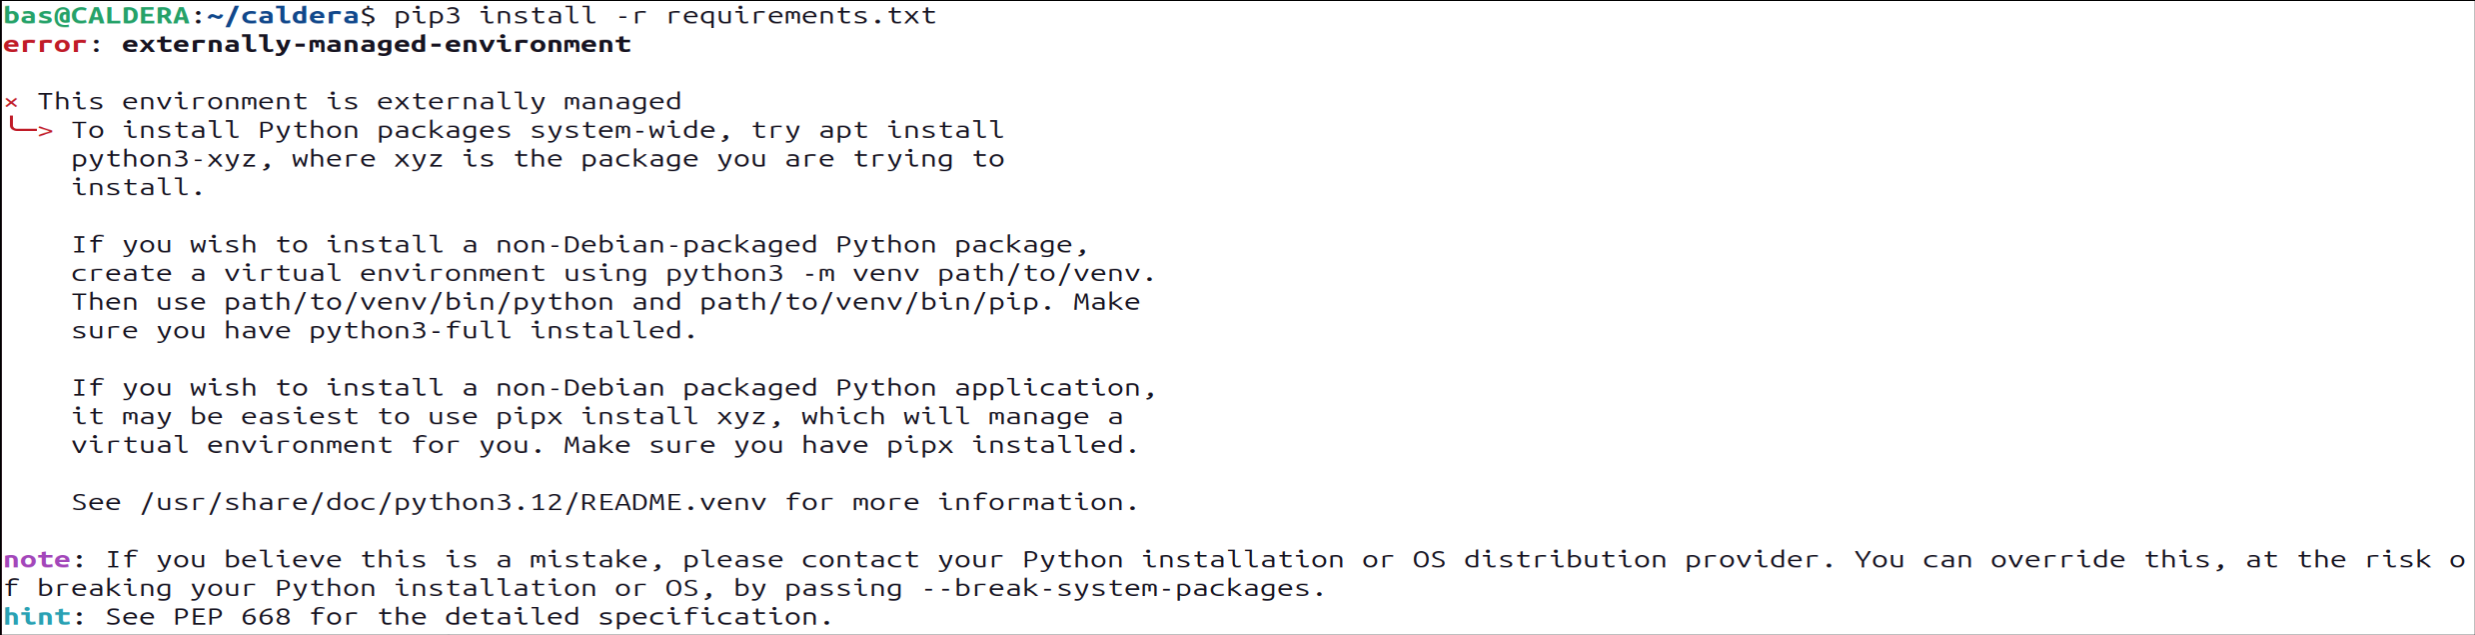
\includegraphics[width=1\textwidth]{figures/Caldera_error.png}
        \caption{Terminal output showing the \texttt{externally-managed-environment} error.}
        \label{fig:venv-error}
    \end{figure}

    \begin{lstlisting}[language=bash, caption={Python Virtual Environment Setup}]
$ sudo apt install python3-pip          # Step 4 [Pkg 2]
$ sudo apt install python3-venv         # Step 5 [Pkg 3]
$ python3 -m venv venv                  # Step 6
$ source venv/bin/activate              # Step 7
$ pip3 install -r requirements.txt      # Step 8
    \end{lstlisting}

    \item \textbf{Build Toolchain Upgrade:} The default Node.js repositories were insufficient for the Vite 7 build engine required by Caldera. The environment was manually upgraded to v22.x to meet the minimum requirement (\texttt{v22.12+}).
    
    \begin{lstlisting}[language=bash, caption={Node.js Toolchain Upgrade}]
$ rm -rf plugins/magma/node_modules     # Step 9
$ sudo apt install curl                 # Step 10 [Pkg 4]
$ curl -fsSL https://deb.nodesource.com/setup_22.x | sudo -E bash - # Step 11
$ sudo apt install npm                  # Step 12 [Pkg 5]
$ sudo apt install -y nodejs            # Step 13 [Pkg 6]
    \end{lstlisting}

    \item \textbf{Execution and Verification:} Finally, the server was compiled and launched to initialize the C2 service.
    
    \begin{lstlisting}[language=bash, caption={Server Compilation and Launch}]
$ python3 server.py --insecure --build  # Step 14
    \end{lstlisting}

    The successful completion of this deployment is confirmed in Figure \ref{fig:caldera_success_install} by the status message ``All systems ready.''
    
    \begin{figure}
        \centering
        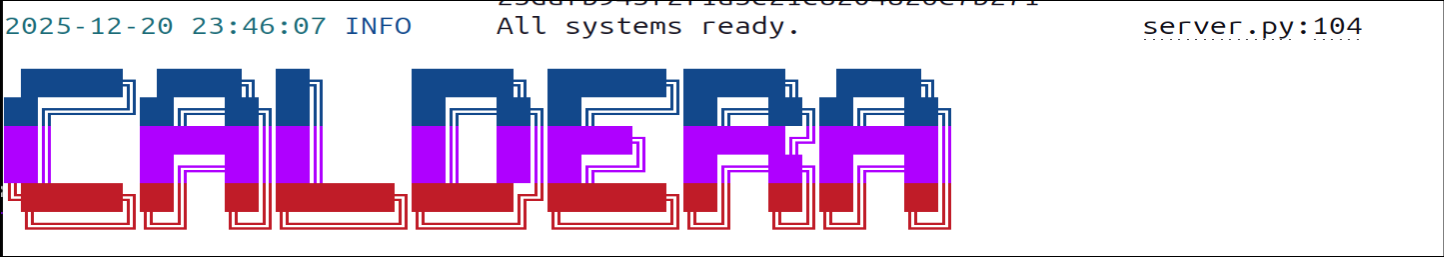
\includegraphics[width=1\textwidth]{figures/caldera_success_install.png}
        \caption{Successful server initialization and build output.}
        \label{fig:caldera_success_install}
    \end{figure}

    The final operational state is confirmed when the administrative login portal becomes accessible (Figure \ref{fig:caldera-interface}).

    \begin{figure}
        \centering
        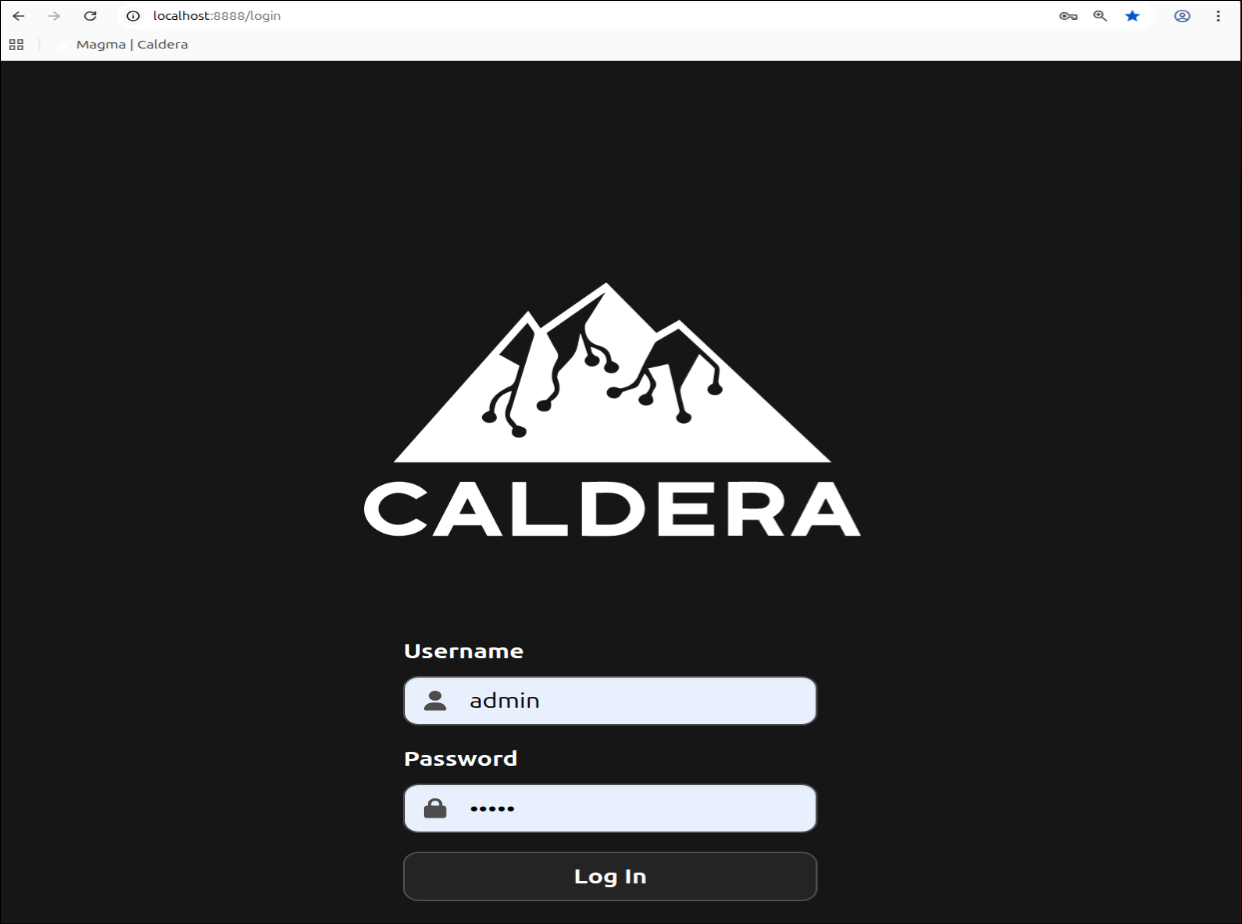
\includegraphics[width=1\textwidth]{figures/caldera_login.png}
        \caption{Caldera administrative login portal.}
        \label{fig:caldera-interface}
    \end{figure}
\end{itemize}

\vspace{1em}
\noindent \textbf{Complexity Metrics Summary:}
\begin{itemize}
    \item \textbf{Total Installation Steps:} 14
    \item \textbf{Total Package Dependencies:} 6
\end{itemize}
        
%% --- SECTION 3: INFECTION MONKEY ---
\subsection{Infection Monkey 's Installation \& Configuration}

The deployment of Infection Monkey focused on establishing the ``Monkey Island'' C2 server. On Ubuntu 24.04, the framework is distributed as an AppImage; however, additional compatibility layers were required to execute the portable binary on a modern kernel.

\begin{itemize}
    \item \textbf{Binary Acquisition and Permissions:} The AppImage (v2.3.0) was retrieved from the official repository. Execution permissions were explicitly granted to the file to allow it to run as a standalone binary.
    
    \begin{lstlisting}[language=bash, caption={Binary Preparation}]
$ chmod u+x InfectionMonkey-v2.3.0.AppImage # Step 1
    \end{lstlisting}

    \item \textbf{Dependency Resolution:} Initial execution attempts failed with a \texttt{dlopen(): error loading libfuse.so.2} error. Modern Ubuntu distributions do not include the FUSE 2 runtime by default, necessitating the installation of the legacy compatibility package.
    
    \begin{lstlisting}[language=bash, caption={Legacy FUSE Support Installation}]
$ sudo apt install libfuse2             # Step 2 [Pkg 1]
    \end{lstlisting}

    \item \textbf{Server Initialization:} The server was manually launched to initialize the Monkey Island backend services. As shown in Figure \ref{fig:monkey-init}, the C2 services successfully started on Port 5000.
    
    \begin{lstlisting}[language=bash, caption={Initial Server Launch}]
$ ./InfectionMonkey-v2.3.0.AppImage     # Step 3
    \end{lstlisting}

    \begin{figure}
        \centering
        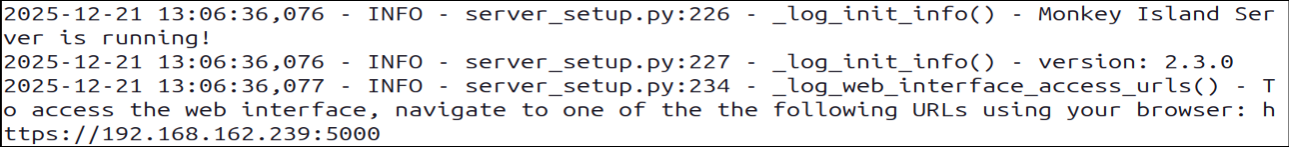
\includegraphics[width=1\textwidth]{figures/monkey_island_logs.png}
        \caption{Terminal output confirming Monkey Island Server is running and accessible via HTTPS.}
        \label{fig:monkey-init}
    \end{figure}

    \item \textbf{Web Interface and Registration:} Upon successful launch, the management console was accessed via a web browser to complete the administrative registration (Figure \ref{fig:monkey-login}).

    \begin{figure}
        \centering
        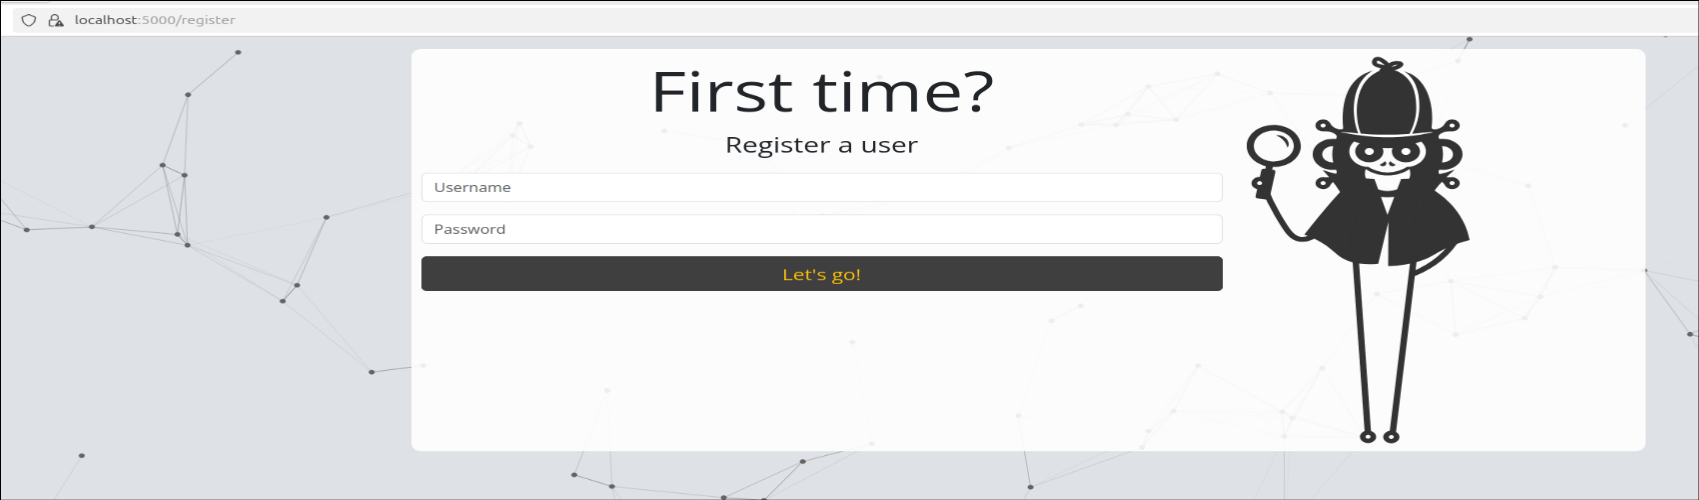
\includegraphics[width=1\textwidth]{figures/monkey_registration.png}
        \caption{Infection Monkey initial user registration interface.}
        \label{fig:monkey-login}
    \end{figure}

    \item \textbf{Persistent Service Configuration:} To ensure the C2 remains active without an open terminal session, the AppImage was registered as a background system service and immediately started.
    
    \begin{lstlisting}[language=bash, caption={System Service Configuration}]
$ ./InfectionMonkey-v2.3.0.AppImage service --install --user bas # Step 4
$ sudo systemctl start infection-monkey # Step 5
    \end{lstlisting}
\end{itemize}

\vspace{1em}
\noindent \textbf{Complexity Metrics Summary:}
\begin{itemize}
    \item \textbf{Total Installation Steps:} 5
    \item \textbf{Total Package Dependencies:} 1
\end{itemize}

%% --- SECTION 4: ATOMIC RED TEAM ---
\subsection{Atomic Red Team 's Installation \& Configuration}

Atomic Red Team provides a library of portable tests mapped to the MITRE ATT\&CK framework. Its execution relies on PowerShell Core, which is not native to Linux and must be installed as a prerequisite.

\begin{itemize}
    \item \textbf{Install PowerShell on Linux:} The installation required registering the proprietary Microsoft package repository before installing the runtime.
    
    \begin{lstlisting}[language=bash, caption={PowerShell Core Installation}]
$ source /etc/os-release
$ wget -q https://packages.microsoft.com/config/ubuntu/$VERSION_ID/packages-microsoft-prod.deb # Step 1
$ sudo dpkg -i packages-microsoft-prod.deb # Step 2
$ sudo apt-get update                   # Step 3
$ sudo apt-get install -y powershell    # Step 4 [Pkg 1]
    \end{lstlisting}

    \item \textbf{Install Execution Framework:} After initializing the PowerShell session, the execution framework and the library of atomic tests (Atomics) were downloaded and installed via the official installation script.
    
    \begin{lstlisting}[language=bash, caption={Framework Installation}]
$ pwsh                                  # Step 5
PS > IEX (IWR 'https://raw.githubusercontent.com/redcanaryco/invoke-atomicredteam/master/install-atomicredteam.ps1' -UseBasicParsing); # Step 6
PS > Install-AtomicRedTeam -getAtomics  # Step 7
    \end{lstlisting}

    As shown in Figure \ref{fig:atomic-success}, the \texttt{Install-AtomicRedTeam} function successfully retrieved the Atomics folder. This process required manual intervention to trust the \textsf{PSGallery} repository.

    \begin{figure}
        \centering
        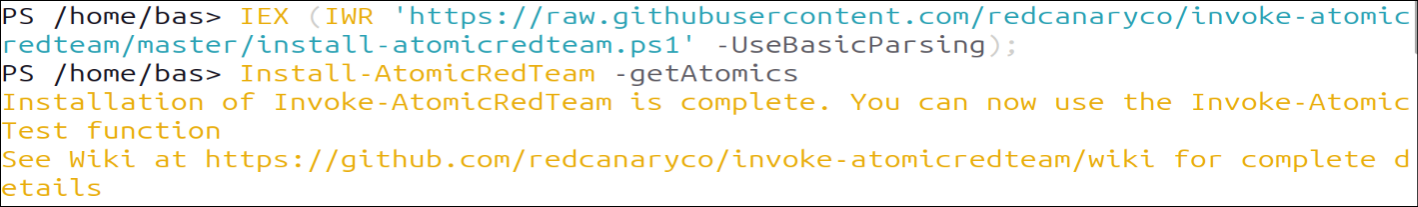
\includegraphics[width=1\textwidth]{figures/atomic-success.png}
        \caption{Output confirming the successful installation of the Atomic Red Team framework and test library.}
        \label{fig:atomic-success}
    \end{figure}

    \item \textbf{Verification:} To confirm operational readiness, the module status was checked to ensure \texttt{Invoke-AtomicRedTeam} was loaded into the session.
    
    \begin{lstlisting}[language=bash, caption={Module Verification}]
PS > Get-Module                         # Step 8
    \end{lstlisting}

    \begin{figure}
        \centering
        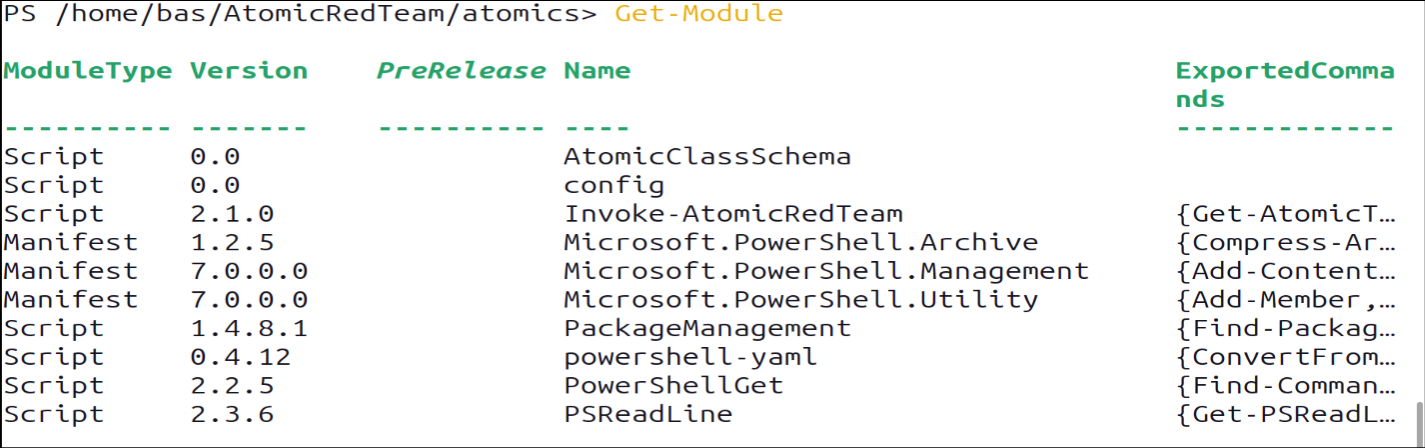
\includegraphics[width=1\textwidth]{figures/atomic-verify.png}
        \caption{Verify the Invoke-AtomicRedTeam module is loaded.}
        \label{fig:atomic-verify}
    \end{figure}
\end{itemize}

\vspace{1em}
\noindent \textbf{Complexity Metrics Summary:}
\begin{itemize}
    \item \textbf{Total Installation Steps:} 8
    \item \textbf{Total Package Dependencies:} 1 (PowerShell Core)
\end{itemize}


%########################################################################%
%#####################|          4.3          |##########################%
%########################################################################%
\section{Attack Simulation Scenarios}\label{sec:AttackScenarios}
To ensure the comparative analysis reflects real-world risk, the attack scenarios for this study were derived using a Threat-Informed Defense approach. We identified high-profile threat actors actively targeting the ASEAN region and global infrastructure in 2025-2026, specifically Mustang Panda\cite{mitre_c0047}\cite{thaicert_mustang}, LockBit\cite{mitre_lockbit}, and Scattered Spider\cite{mitre_c0027}.

To validate the statistical relevance of our selection, we prioritized techniques based on the \textbf{Center for Threat-Informed Defense (CTID) Sightings Ecosystem} (v2.0) \cite{ctid_sightings}. From this global high-prevalence list, we selected 20 specific sub-techniques and adapted them for a \textbf{hybrid multi-victim testbed (Windows and Linux)}, reflecting the cross-platform nature of modern campaigns.

For the purpose of this comparative analysis, these twenty distinct attack simulations are indexed as \textbf{S1} through \textbf{S20} (Scenario 1 to Scenario 20). This indexing system is used throughout the experimental results and the evaluation matrix to facilitate concise cross-referencing. The scenarios are detailed below, categorized by their CTID global prevalence ranking:

% --- RANK 1 ---
\subsection{CTID Rank \#1: Command and Scripting Interpreter (T1059)}
\begin{itemize}
    \item \textbf{S1: PowerShell Execution (Windows)} \\
    \textbf{Technique:} T1059.001 (PowerShell) \\
    \textbf{Origin:} Mustang Panda. \\
    \textbf{Description:} Simulates ``Living-off-the-Land'' by executing Base64-encoded commands directly in memory using \texttt{powershell.exe -enc}, bypassing file-based scanning.

    \item \textbf{S2: Bash Script Execution (Linux)} \\
    \textbf{Technique:} T1059.004 (Unix Shell) \\
    \textbf{Origin:} Mustang Panda (Linux VShell) / LockBit Linux. \\
    \textbf{Description:} Executes a malicious bash script downloaded from a remote source (e.g., \texttt{curl | bash}), a common entry vector for Linux backdoors.
\end{itemize}

% --- RANK 2 ---
\subsection{CTID Rank \#2: Scheduled Task/Job (T1053)}
\begin{itemize}
    \item \textbf{S3: Scheduled Task Creation (Windows)} \\
    \textbf{Technique:} T1053.005 (Scheduled Task) \\
    \textbf{Origin:} LockBit. \\
    \textbf{Description:} Uses \texttt{schtasks.exe} to create a task that runs a payload at system startup, testing persistence detection.

    \item \textbf{S4: Cron Job Persistence (Linux)} \\
    \textbf{Technique:} T1053.003 (Cron) \\
    \textbf{Origin:} LockBit Linux / Scattered Spider. \\
    \textbf{Description:} Appends a malicious entry to the user's crontab (e.g., \texttt{echo "* * * * * /tmp/malware" >> /var/spool/cron/root}) to maintain persistence after reboot.
\end{itemize}

% --- RANK 3 ---
\subsection{CTID Rank \#3: Hijack Execution Flow (T1574)}
\begin{itemize}
    \item \textbf{S5: DLL Side-Loading (Windows)} \\
    \textbf{Technique:} T1574.002 (DLL Side-Loading) \\
    \textbf{Origin:} Mustang Panda (PlugX). \\
    \textbf{Description:} Places a malicious DLL alongside a legitimate, signed executable. When run, the trusted app loads the malware, testing signature-based trust models.
\end{itemize}

% --- RANK 4 ---
\subsection{CTID Rank \#4: Impair Defenses (T1562)}
\begin{itemize}
    \item \textbf{S6: Disable Security Tools (Windows)} \\
    \textbf{Technique:} T1562.001 (Disable Tools) \\
    \textbf{Origin:} LockBit. \\
    \textbf{Description:} Attempts to stop the Windows Defender service (\texttt{Windefend}) or modify registry keys to disable Real-Time Monitoring.

    \item \textbf{S7: Indicator Removal: Clear Logs (Linux)} \\
    \textbf{Technique:} T1070.002 (Clear Linux Logs) \\
    \textbf{Origin:} Scattered Spider. \\
    \textbf{Description:} Deletes critical log files (e.g., \texttt{rm /var/log/auth.log}) and clears shell history (\texttt{history -c}), attempting to blind forensic analysis.
\end{itemize}

% --- RANK 5 ---
\subsection{CTID Rank \#5: Masquerading (T1036)}
\begin{itemize}
    \item \textbf{S8: Match Legitimate Name (Windows)} \\
    \textbf{Technique:} T1036.005 (Match Legitimate Name) \\
    \textbf{Origin:} Mustang Panda (SnakeDisk). \\
    \textbf{Description:} Renames a malicious binary to a system filename (e.g., \texttt{svchost.exe}) and executes it from a temporary folder.

    \item \textbf{S9: Hidden Files and Directories (Linux)} \\
    \textbf{Technique:} T1564.001 (Hidden Files) \\
    \textbf{Origin:} LockBit Linux / General. \\
    \textbf{Description:} Hides a malicious payload by prepending a dot to the filename (e.g., \texttt{/tmp/.malware}), testing if the endpoint sensor monitors hidden artifacts.
\end{itemize}

% --- RANK 10 ---
\subsection{CTID Rank \#10: Remote Services (Lateral Movement) (T1021)}
\begin{itemize}
    \item \textbf{S10: Lateral Movement via SMB (Windows)} \\
    \textbf{Technique:} T1021.002 (SMB/Windows Admin Shares) \\
    \textbf{Origin:} LockBit. \\
    \textbf{Description:} Simulates lateral propagation by connecting to a secondary Windows victim via SMB (Admin Shares) using compromised credentials.

    \item \textbf{S11: SSH Lateral Movement (Linux)} \\
    \textbf{Technique:} T1021.004 (SSH) \\
    \textbf{Origin:} Scattered Spider / LockBit. \\
    \textbf{Description:} Uses a stolen SSH key or credentials to remotely execute commands on a neighboring Linux VM, testing internal network segmentation visibility.
\end{itemize}

% --- RANK 13 ---
\subsection{CTID Rank \#13: Credential Access (T1003)}
\begin{itemize}
    \item \textbf{S12: OS Credential Dumping (Windows)} \\
    \textbf{Technique:} T1003.001 (LSASS Memory) \\
    \textbf{Origin:} Scattered Spider. \\
    \textbf{Description:} Uses \texttt{procdump} to dump the memory of \texttt{lsass.exe}, attempting to harvest NTLM hashes.

    \item \textbf{S13: Credential Dumping: Shadow/SSH (Linux)} \\
    \textbf{Technique:} T1003.008 (Text Files) \\
    \textbf{Origin:} Scattered Spider. \\
    \textbf{Description:} Attempts to read sensitive credential files such as \texttt{/etc/shadow} (password hashes) or \texttt{\textasciitilde/.ssh/id\_rsa} (private keys).
\end{itemize}

% --- RANK 14 ---
\subsection{CTID Rank \#14: System Information Discovery (T1082)}
\begin{itemize}
    \item \textbf{S14: System Discovery (Windows)} \\
    \textbf{Technique:} T1082 (System Info Discovery) \\
    \textbf{Origin:} Mustang Panda. \\
    \textbf{Description:} Runs \texttt{systeminfo} and \texttt{tasklist} to profile the endpoint environment.

    \item \textbf{S15: System Discovery (Linux)} \\
    \textbf{Technique:} T1082 (System Info Discovery) \\
    \textbf{Origin:} LockBit Linux. \\
    \textbf{Description:} Executes enumeration commands like \texttt{uname -a}, \texttt{id}, and \texttt{lscpu} to identify the kernel version and user privileges.
\end{itemize}

% --- RANK 15 ---
\subsection{CTID Rank \#15: Data Encrypted for Impact (T1486)}
\begin{itemize}
    \item \textbf{S16: Bulk File Encryption (Windows)} \\
    \textbf{Technique:} T1486 (Data Encrypted for Impact) \\
    \textbf{Origin:} LockBit 3.0. \\
    \textbf{Description:} Simulates ransomware by rapidly encrypting a folder of documents on Windows using a high-entropy algorithm.

    \item \textbf{S17: Bulk File Encryption (Linux)} \\
    \textbf{Technique:} T1486 (Data Encrypted for Impact) \\
    \textbf{Origin:} LockBit Linux/ESXi Variant. \\
    \textbf{Description:} Simulates the Linux variant of LockBit by encrypting files in the \texttt{/home} directory, testing behavioral detection on Linux.
\end{itemize}

% --- ADDITIONAL ---
\subsection{Additional Cross-Platform Techniques}
\begin{itemize}
    \item \textbf{S18: Ingress Tool Transfer (Mixed)} \\
    \textbf{Technique:} T1105 (Ingress Tool Transfer) \\
    \textbf{Origin:} All Actors. \\
    \textbf{Description:} Downloads a payload using native tools: \texttt{certutil} (Windows) or \texttt{wget/curl} (Linux).

    \item \textbf{S19: SSH Authorized Keys Persistence (Linux)} \\
    \textbf{Technique:} T1098.004 (SSH Authorized Keys) \\
    \textbf{Origin:} Scattered Spider. \\
    \textbf{Description:} Adds a new public key to \texttt{\textasciitilde/.ssh/authorized\_keys} to maintain persistent remote access.

    \item \textbf{S20: Exfiltration Over C2 Channel (Mixed)} \\
    \textbf{Technique:} T1041 (Exfiltration Over C2) \\
    \textbf{Origin:} Mustang Panda. \\
    \textbf{Description:} Simulates data theft by sending dummy data to an external IP via HTTP POST.
\end{itemize}

%######################################################
%########|   List of Selected Attack Simulation Scenarios  |#############
%######################################################
\begin{table}
    \centering
    \caption{List of Selected Attack Simulation Scenarios (Windows \& Linux)}
    \label{tab:attack_scenarios}
    \renewcommand{\arraystretch}{1.2}
    \begin{tabular}{|c|p{3.8cm}|c|c|p{3.5cm}|}
    \hline
    \textbf{ID} & \textbf{Scenario Name} & \textbf{Rank} & \textbf{OS Target} & \textbf{Primary Threat Actor} \\ \hline
    S1 & PowerShell Execution & 1 & Windows & Mustang Panda \\ \hline
    S2 & Bash Script Execution & 1 & Linux & Mustang Panda, LockBit \\ \hline
    S3 & Scheduled Task & 2 & Windows & LockBit \\ \hline
    S4 & Cron Job Persistence & 2 & Linux & LockBit \\ \hline
    S5 & DLL Side-Loading & 3 & Windows & Mustang Panda \\ \hline
    S6 & Disable Security Tools & 4 & Windows & LockBit \\ \hline
    S7 & Clear Logs (History) & 4 & Linux & Scattered Spider \\ \hline
    S8 & Masquerading (Name) & 5 & Windows & Mustang Panda \\ \hline
    S9 & Hidden Files (.file) & 5 & Linux & LockBit \\ \hline
    S10 & SMB Lateral Movement & 10 & Windows & LockBit \\ \hline
    S11 & SSH Lateral Movement & 10 & Linux & Scattered Spider \\ \hline
    S12 & LSASS Dumping & 13 & Windows & Scattered Spider \\ \hline
    S13 & Dump Shadow/Keys & 13 & Linux & Scattered Spider \\ \hline
    S14 & System Discovery & 14 & Windows & Mustang Panda \\ \hline
    S15 & System Discovery & 14 & Linux & LockBit \\ \hline
    S16 & Data Encryption & 15 & Windows & LockBit \\ \hline
    S17 & Data Encryption & 15 & Linux & LockBit \\ \hline
    S18 & Ingress Tool Transfer & - & Mixed & All Actors \\ \hline
    S19 & SSH Key Persistence & - & Linux & Scattered Spider \\ \hline
    S20 & Exfiltration Over C2 & - & Windows \& Linux & Mustang Panda \\ \hline
    \end{tabular}
\end{table}

%================================= Usability & Deployment Complexity

\section{Usability \& Deployment Complexity}\label{sec:Matrix1}
\subsection{Number of installation steps required}\label{sec:Matrix1_1_1}

Deployment friction was quantified by walking each tool's official installation documentation end-to-end and counting every discrete required action (cloning the repository, installing a runtime, running a setup script, editing a configuration file, and starting a service each counted as one step). MITRE Caldera required 14 steps, driven primarily by its Python virtual-environment setup and the need to individually initialize its bundled plugin submodules. Atomic Red Team required 8 steps, centered on its PowerShell installer script and the separate checkout of the atomics test library. Infection Monkey required only 5 steps, reflecting its single self-contained AppImage/Docker distribution model, which collapses most of the setup Caldera and Atomic Red Team require into a single download-and-run action.

\subsection{Dependency requirements}\label{sec:Matrix1_1_2}

Dependency weight was assessed by counting the distinct external runtime packages each tool's own manifest (or documentation) declares as required, excluding vendored or bundled libraries. MITRE Caldera declared 6 packages, reflecting its Python application-server stack and plugin-specific requirements. Infection Monkey and Atomic Red Team each declared a single external dependency --- Infection Monkey ships as a self-contained AppImage/container image, and Atomic Red Team requires only PowerShell 5.1+ (or PowerShell Core), with any additional tooling scoped to individual atomic tests rather than the framework itself.

\begin{table}
    \centering
    \caption{Phase 2 Evaluation: Sub-criterion Scoring Comparison}
    \small
    \begin{tabularx}{\textwidth}{lXXX}
        \toprule
        \textbf{Sub-criterion} & \textbf{MITRE Caldera} & \textbf{Infection Monkey} & \textbf{Atomic Red Team} \\
        \midrule
        1.1 Number of installation steps required & 1 (14 steps) & 3 (5 steps) & 2 (8 steps) \\
        \addlinespace
        1.2 Dependency requirements & 1 (6 packages) & 3 (1 package) & 3 (1 package) \\
        \midrule
        \textbf{Average} & \textbf{1.00} & \textbf{3.00} & \textbf{2.50} \\
        \bottomrule
    \end{tabularx}
\end{table}

Taken together, Infection Monkey presents the lowest deployment barrier of the three tools, while MITRE Caldera's more sophisticated multi-agent, multi-plugin architecture comes at the cost of a heavier and more involved installation process --- a trade-off consistent with prior comparative work on open-source adversary-emulation tooling~\cite{landauer2024}.

%================================= Threat Intelligence Alignment \& Maintenance

\section{Threat Intelligence Alignment \& Maintenance}\label{sec:Matrix2}
\subsection{Frequency of MITRE ATT\&CK techniques update}\label{sec:Update_frequency}

Update frequency was measured via a live pull of each tool's GitHub commit history as of the evaluation date. Atomic Red Team was the most actively updated of the three, with 119 commits in the preceding twelve months (an average of 9.92 per month) and a most recent commit only two days prior to measurement. MITRE Caldera, measured at the ecosystem level (its main repository plus 14 distributed plugin submodules, per the methodological discussion in Section~\ref{sec:Matrix6}), recorded 341 commits over the same period. Infection Monkey recorded zero commits in the preceding twelve months, its last commit dating to 24 July 2024 --- consistent with the project's effective dormancy since release v2.3.0. Both Caldera and Atomic Red Team therefore score [3]~Frequent, while Infection Monkey scores [0]~Static.

\subsection{Update method}\label{sec:Update_method}
A notable framework-level finding for sub-criterion 2.2 is that none of the three evaluated tools provides automated MITRE ATT\&CK content synchronization. The two actively-maintained platforms (MITRE Caldera and Atomic Red Team) both require manual operator intervention --- a \texttt{git pull} or a re-execution of the install script --- to apply new content. Neither offers scheduled background updates, nor immediate synchronization with MITRE's quarterly ATT\&CK release cadence. Infection Monkey lacks any update mechanism beyond replacing the AppImage binary. This represents a categorical gap between open-source and commercial BAS platforms, where automated content synchronization is typically advertised as a key differentiator. The implication for operational deployment is that operators of open-source BAS tooling must establish their own update cadence to ensure ongoing alignment with current threat intelligence.

\begin{table}
    \centering
    \caption{Phase 2 Evaluation: Sub-criterion Scoring Comparison}
    \small
    \begin{tabularx}{\textwidth}{lXXX}
        \toprule
        \textbf{Sub-criterion} & \textbf{MITRE Caldera} & \textbf{Infection Monkey} & \textbf{Atomic Red Team} \\
        \midrule
        2.1 Frequency of MITRE ATT\&CK techniques update & 3 (341/yr\textsuperscript{a}) & 0 (0/yr) & 3 (119/yr) \\
        \addlinespace
        2.2 Update method & 1 (manual git pull) & 0 (no mechanism) & 1 (manual re-install) \\
        \midrule
        \textbf{Average} & \textbf{2.00} & \textbf{0.00} & \textbf{2.00} \\
        \bottomrule
    \end{tabularx}
    \\[4pt]
    \footnotesize\textsuperscript{a}Caldera measured at the ecosystem level (main repository plus 14 plugin submodules); the single-repository count is only 34 commits/yr, which is methodologically misleading for a distributed-plugin architecture (see Section~\ref{sec:Matrix6}).
\end{table}


%========= Scenario Coverage, Reliability & Relevance ===========
\section{Scenario Coverage, Reliability \& Relevance}\label{sec:Matrix3}
\subsection{Number of Supported MITRE ATT\&CK Techniques}\label{sec:results_im_3_1}

This subsection presents the breadth of MITRE ATT\&CK coverage provided by each of the three selected tools as deployed in the laboratory
environment. Coverage was determined by extracting every technique and sub-technique
identifier from each tool's raw ability and configuration files, then cross-referencing each identifier against the official MITRE ATT\&CK Enterprise matrix, version~19.2 (downloaded directly from MITRE on 7 September 2026), which comprises \textbf{697 valid, non-deprecated techniques and sub-techniques} (222 top-level techniques plus 475 sub-techniques) and forms the reference population against which each tool's coverage is assessed in this study. Both parent techniques and their sub-techniques were counted individually
(e.g.\ T1110, T1110.001, T1110.003, and T1110.004 are each recorded as distinct entries), reflecting the granularity at which each tool implements and reports adversarial behaviors. An identifier claimed by a tool but no longer present under that exact identifier in v19.2 --- because MITRE has since deprecated, merged, or renumbered it (for example, the \texttt{T1562} ``Impair Defenses'' family was renumbered to \texttt{T1685} in ATT\&CK~v19) --- was excluded from that tool's count, since it no longer represents a technique the tool can be credited with covering under the current framework.

MITRE Caldera covers 320 of the 697 valid v19.2 techniques (45.9\%), Atomic Red Team covers 317 (45.5\%), and Infection Monkey covers 19 (2.7\%). Both Caldera and Atomic Red Team therefore fall in the [2]~Moderate band (25--50\% coverage), while Infection Monkey falls in the [0]~Minimal band ($<$10\% coverage) --- a consequence of its technique mapping predating ATT\&CK's 2020 sub-technique restructuring and never having been updated to the current identifier scheme.

\subsection{High-Probability Threat Alignment}\label{sec:results_im_3_2}

Whereas Section~\ref{sec:results_im_3_1} measures raw breadth of ATT\&CK coverage, this sub-criterion measures whether each tool covers the 20 high-probability, threat-actor-mapped scenarios (S1--S20, Table~\ref{tab:attack_scenarios}) prioritized for this study from the MITRE Center for Threat-Informed Defense (CTID) top-technique rankings and tied to the Mustang Panda, LockBit, and Scattered Spider TTP profiles introduced in Section~\ref{sec:AttackScenarios}. MITRE Caldera and Atomic Red Team each structurally support 19 of the 20 scenarios (95\%), missing only S5 (T1574.002, DLL Side-Loading), and both therefore score [3]~High Alignment. Infection Monkey supports only 6 of the 20 scenarios (30\%) --- S1, S10, S11, S16, S17, and S18 --- missing every Linux-specific persistence and discovery scenario (S2, S4, S7, S9, S11 excepted, S13, S15), the LSASS credential-dumping scenario (S12), the SSH-key persistence scenario (S19), and the C2-exfiltration scenario (S20). This is a structural scope gap in Infection Monkey's exploiter and post-breach-action library rather than an execution failure, and Infection Monkey therefore scores [1]~Inadequate.

\subsection{Execution reliability}\label{sec:results_im_3_3}

Execution reliability is the primary metric of this study: whether an attempted technique genuinely reached and executed against the intended victim, evidenced by a completion signal specific to each tool's architecture (a full agent round-trip for MITRE Caldera; \texttt{Executing test:} followed by an \texttt{Exit code:} for Atomic Red Team; a technique-specific exploitation or propagation event for Infection Monkey). Reliability was measured across the 19 techniques common to all three tools' campaigns, each run 10 times, for 190 total runs per tool. MITRE Caldera achieved 188/190 successful runs (98.9\%), Atomic Red Team achieved 189/190 (99.5\%), and Infection Monkey achieved 150/190 (78.9\%); all three therefore score [3]~Highly Reliable ($>$75\% success).

Every non-successful run was individually root-caused rather than treated as an undifferentiated failure. MITRE Caldera's two initial non-passing techniques (T1021.002 and T1021.006, lateral movement via SMB and WinRM) were traced to a harness configuration gap --- the CALDERA server lacked a fact source providing the credential and remote-target values its abilities require --- and both reached 10/10 genuine command executions once a proper fact source was supplied, independently confirmed via the victim's own Security and Sysmon event logs. Infection Monkey's non-passing techniques fall into three distinct categories: T1021.001 (RDP) is a confirmed software defect, its RDP exploiter crashing as a subprocess before ever attempting a connection, traced to a PyInstaller frozen-executable interaction with Python's \texttt{spawn} multiprocessing start method; T1003 (OS credential dumping) is a capability-and-environment limitation, since the propagated agent runs without administrative privileges and the target lab has no domain controller for its Zerologon exploiter to target; and detection of T1071.001, although unrelated to execution reliability itself, was separately found to be a fixable Splunk detection-rule defect (the saved search matched on a Sysmon-specific field name that this activity's Security-log events do not populate), corrected during this study.

%%%%%%%%%%%%%%%%%%%%%%%%%%%%%%%%%%%%%%%%%%%%%%%%%%%%%%%%%%%%%%%%%%%%

\section{Operational Performance \& Output Quality}\label{sec:Matrix4}

\subsection{CPU usage of BAS server }\label{sec:Matrix4_4_1}

CPU overhead was measured as each BAS server host's mean CPU utilization during the full campaign's continuous sampling window, expressed as percentage points above that same host's idle baseline. MITRE Caldera showed the smallest overhead of the three tools at +2.83 points, followed by Atomic Red Team at +12.12 points; both fall well within the [3]~Minimal band ($<$15\% overhead). Infection Monkey showed the largest overhead at +18.43 points, placing it in the [2]~Moderate band (15--40\%). A caveat on this comparison is that Atomic Red Team's ``server'' is architecturally a lightweight PowerShell/WinRM command runner on the controller host, whereas MITRE Caldera and Infection Monkey each run a full C2/Island server process; this architectural difference is partly a category distinction rather than a pure measure of code efficiency, and tends to structurally favor Atomic Red Team's figures.

\subsection{Memory usage of BAS server}\label{sec:Matrix4_im_4_2}

Memory overhead was measured using the same continuous-sampling methodology as Section~\ref{sec:Matrix4_4_1}, expressed as percentage points above each host's idle memory baseline. All three tools fall in the [3]~Minimal band ($<$15\% overhead): MITRE Caldera at +1.29 points, Atomic Red Team at +2.48 points, and Infection Monkey at +13.33 points. The same architectural caveat noted for CPU overhead applies here.

\subsection{Quality of reports}\label{sec:Matrix4_4_3}

Report quality was assessed by generating each tool's native output artifact after a completed campaign run and comparing its content against four fixed bands ranging from raw CLI output to specific, actionable remediation guidance. MITRE Caldera produces a structured Operation Report with event logs and named ATT\&CK-technique mitigation guidance, though without machine-actionable detection content such as Snort or Sigma rules, placing it in the [2]~General Advice band. Infection Monkey produces a Security Report with a dedicated ``Machine-related Recommendations'' section offering comparable named mitigation steps, likewise scoring [2]~General Advice. Atomic Red Team emits only raw PowerShell or SSH standard output with no synthesized report file, scoring [0]~No Reports. This result should be read alongside Atomic Red Team's explicit design philosophy as a composable atomic-test executor intended to be wrapped by external tooling (for example, feeding results to a SIEM) rather than to function as a standalone reporting platform; the criterion, as constructed, penalizes this design choice relative to the two all-in-one platforms.

\begin{table}
    \centering
    \caption{Phase 2 Evaluation: Sub-criterion Scoring Comparison}
    \small
    \begin{tabularx}{\textwidth}{lXXX}
        \toprule
        \textbf{Sub-criterion} & \textbf{MITRE Caldera} & \textbf{Infection Monkey} & \textbf{Atomic Red Team} \\
        \midrule
        4.1 CPU usage of BAS server & 3 (+2.83 pts) & 2 (+18.43 pts) & 3 (+12.12 pts) \\
        \addlinespace
        4.2 Memory usage of BAS server & 3 (+1.29 pts) & 3 (+13.33 pts) & 3 (+2.48 pts) \\
        \addlinespace
        4.3 Quality of reports & 2 (mapped mitigations) & 2 (mitigation recs) & 0 (raw stdout only) \\
        \midrule
        \textbf{Average} & \textbf{2.67} & \textbf{2.33} & \textbf{2.00} \\
        \bottomrule
    \end{tabularx}
\end{table}

\section{Framework Extensibility \& Custom Scenario Creation}\label{sec:Matrix5}

\subsection{Add/modify attack scenarios}\label{sec:Matrix5_5_1}

This sub-criterion evaluates the mechanism each tool provides for an operator to add or edit an attack scenario. MITRE Caldera provides both YAML-defined ability files and a dedicated ``Create an Ability'' graphical interface, requiring no programming to author a new scenario, and scores [3]~Easy. Atomic Red Team similarly uses a simple, documented YAML schema per atomic test with no coding required for a standard test, also scoring [3]~Easy. Infection Monkey supports extension only through uploading a compiled plugin package (\texttt{.tar}) via its graphical interface; authoring a new plugin, however, requires Python development against Infection Monkey's plugin architecture, placing it in the [2]~Possible (code required) band.

\subsection{Ease of creating custom TTPs}\label{sec:Matrix5_5_2}

This sub-criterion evaluates how easily an operator can chain multiple techniques into a single coordinated multi-step scenario, distinct from Section~\ref{sec:Matrix5_5_1}'s more basic question of whether a scenario can be authored at all. MITRE Caldera provides Adversary Profiles and Planners that chain individual Abilities into a custom operational sequence entirely through its graphical interface, scoring [3]~User-Friendly. Atomic Red Team's atomics are discrete, single-step tests by design; chaining several into a multi-stage scenario requires external scripting, such as an operator-written PowerShell loop over a sequence of test IDs, placing it in the [2]~Requires Scripting band. Infection Monkey offers no built-in composition mechanism across its fixed exploiter set --- chaining custom multi-stage behavior would require deep changes to its plugin architecture rather than any user-facing configuration --- and it therefore scores [1]~Complex/Undocumented.

\begin{table}
    \centering
    \caption{Phase 2 Evaluation: Sub-criterion Scoring Comparison}
    \small
    \begin{tabularx}{\textwidth}{lXXX}
        \toprule
        \textbf{Sub-criterion} & \textbf{MITRE Caldera} & \textbf{Infection Monkey} & \textbf{Atomic Red Team} \\
        \midrule
        5.1 Add/modify attack scenarios & 3 (YAML + GUI) & 2 (plugin, needs Python) & 3 (YAML, no coding) \\
        \addlinespace
        5.2 Ease of creating custom TTPs & 3 (GUI Planners) & 1 (no composition) & 2 (ext.\ scripting) \\
        \midrule
        \textbf{Average} & \textbf{3.00} & \textbf{1.50} & \textbf{2.50} \\
        \bottomrule
    \end{tabularx}
\end{table}

\section{Community Health \& Project Maturity}\label{sec:Matrix6}

The Criterion~6 measurements reveal a clear three-tier stratification of project 
maturity across the evaluated tools, and confirm one of the central findings 
informing the Phase~1 down-selection in Chapter~3. \textbf{Atomic Red Team} leads on every 
quantitative community metric --- stars (11,895), forks (3,107), all-time 
contributors (498), and active contributors in the past twelve months (35). 
\textbf{MITRE Caldera}, when measured at the ecosystem level (main repository plus the 
14 distributed plugin submodules), records the highest raw commit volume of the 
three tools (341 commits over twelve months versus Atomic Red Team's 185), but with 
a smaller active-contributor pool (21 versus 35). \textbf{Infection Monkey} records 
substantial historical accumulation (6,998 stars and 77 all-time contributors) 
but zero contributors active in the past twelve months and 238 unaddressed open 
issues, consistent with the project's effective dormancy since v2.3.0 in 
September~2023.

The Caldera measurement also illustrates a methodological point worth surfacing 
explicitly. Caldera's main-branch git history shows only 34~commits in the past 
twelve months, none in the past three months --- a pattern that, taken 
in isolation, would suggest project stagnation. The submodule-aware measurement 
reveals the opposite: 175~commits in the past three months alone, distributed 
across the plugin ecosystem, and 12 of 14 plugins updated within the past 
60~days. Single-repository commit counts are not, by themselves, a reliable 
indicator of maintenance pace for projects that follow a distributed plugin 
architecture.
\begin{figure}
    \centering
    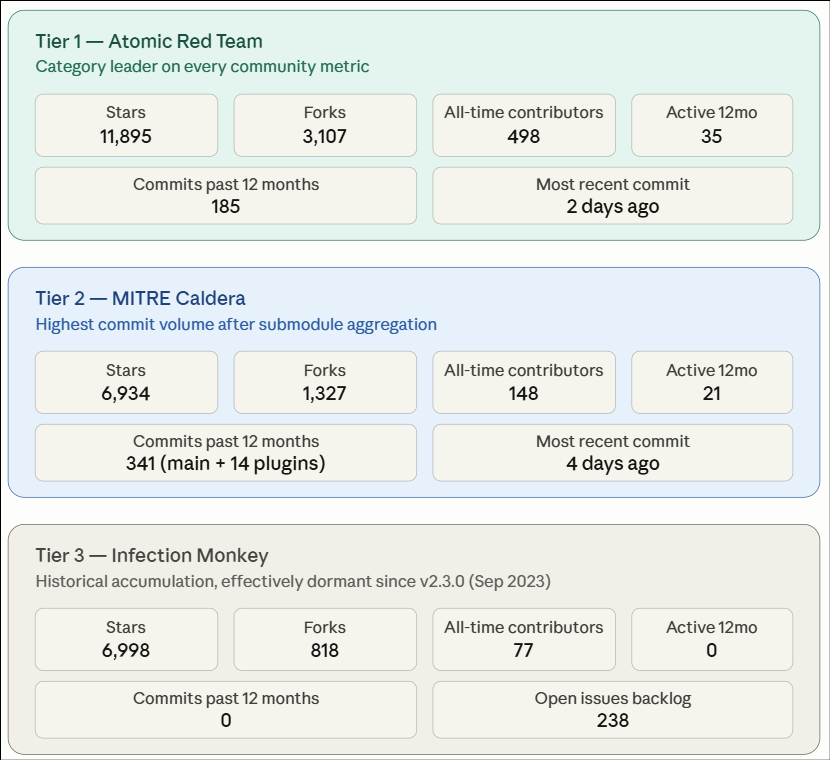
\includegraphics[width=1\linewidth]{figures/Community health and project maturity.png}
    \caption{Community health and project maturity  }
    \label{fig:Community}
\end{figure}

%########################################################################%
%###################|          4.4          |############################%
%########################################################################%

\begin{table}
    \caption{Comparison of breach and attack simulation frameworks}
    \label{tab:results_comparison}
    \centering
    \renewcommand{\arraystretch}{1.3}
    \begin{tabular}{|p{0.50\linewidth}|>{\centering\arraybackslash}p{2cm}|>{\centering\arraybackslash}p{2cm}|>{\centering\arraybackslash}p{2cm}|}
        \hline
        \textbf{Criterion} & \textbf{MITRE Caldera} & \textbf{Infection Monkey} & \textbf{Atomic Red Team} \\ \hline
        
        \multicolumn{4}{|l|}{\textbf{1. Usability \& Deployment Complexity}} \\ \hline
        1.1 Number of installation steps required & 1 \newline \footnotesize{(14)} & 3 \newline \footnotesize{(5)} & 2 \newline \footnotesize{(8)} \\ \hline
        1.2 Dependency requirements & 1 \newline \footnotesize{(6 pkgs)} & 3 \newline \footnotesize{(1 pkg)} & 3 \newline \footnotesize{(1 pkg)} \\ \hline
        \textit{Average} & \textit{1.00} & \textit{3.00} & \textit{2.50} \\ \hline
        
        \multicolumn{4}{|l|}{\textbf{2. Threat Intelligence Alignment \& Maintenance}} \\ \hline
        2.1 Frequency of MITRE ATT\&CK techniques update & 3 \newline \footnotesize{(341/yr\textsuperscript{a})} & 0 \newline \footnotesize{(0/yr)} & 3 \newline \footnotesize{(119/yr)} \\ \hline
        2.2 Update method & 1 \newline \footnotesize{(manual)} & 0 \newline \footnotesize{(none)} & 1 \newline \footnotesize{(manual)} \\ \hline
        \textit{Average} & \textit{2.00} & \textit{0.00} & \textit{2.00} \\ \hline
        
        \multicolumn{4}{|l|}{\textbf{3. Scenario Coverage, Reliability \& Relevance}} \\ \hline
        3.1 Number of supported MITRE ATT\&CK techniques (of 697 valid v19.2 techniques) & 2 \newline \footnotesize{(320/697 = 45.9\%)} & 0 \newline \footnotesize{(19/697 = 2.7\%)} & 2 \newline \footnotesize{(317/697 = 45.5\%)} \\ \hline
        3.2 High-Probability Threat Alignment (CTID top-20) & 3 \newline \footnotesize{(19/20 = 95\%)} & 1 \newline \footnotesize{(6/20 = 30\%)} & 3 \newline \footnotesize{(19/20 = 95\%)} \\ \hline
        3.3 Execution reliability (Attack Rate) & 3 \newline \footnotesize{(98.9\%, 188/190)} & 3 \newline \footnotesize{(78.9\%, 150/190)} & 3 \newline \footnotesize{(99.5\%, 189/190)} \\ \hline
        \textit{Average} & \textit{2.67} & \textit{1.33} & \textit{2.67} \\ \hline

        \multicolumn{4}{|l|}{\textbf{4. Operational Performance \& Output Quality}} \\ \hline
        4.1 CPU usage of BAS server (vs.\ idle baseline) & 3 \newline \footnotesize{(+2.83 pts)} & 2 \newline \footnotesize{(+18.43 pts)} & 3 \newline \footnotesize{(+12.12 pts)} \\ \hline
        4.2 Memory usage of BAS server (vs.\ idle baseline) & 3 \newline \footnotesize{(+1.29 pts)} & 3 \newline \footnotesize{(+13.33 pts)} & 3 \newline \footnotesize{(+2.48 pts)} \\ \hline
        4.3 Quality of reports & 2 \newline \footnotesize{(mapped mitigations)} & 2 \newline \footnotesize{(mitigation recs)} & 0 \newline \footnotesize{(raw stdout only)} \\ \hline
        \textit{Average} & \textit{2.67} & \textit{2.33} & \textit{2.00} \\ \hline

        \multicolumn{4}{|l|}{\textbf{5. Framework Extensibility \& Custom Scenario Creation}} \\ \hline
        5.1 Add/modify attack scenarios & 3 \newline \footnotesize{(YAML + GUI)} & 2 \newline \footnotesize{(plugin, needs Python)} & 3 \newline \footnotesize{(YAML, no coding)} \\ \hline
        5.2 Ease of creating custom TTPs & 3 \newline \footnotesize{(GUI Planners)} & 1 \newline \footnotesize{(no composition)} & 2 \newline \footnotesize{(ext.\ scripting)} \\ \hline
        \textit{Average} & \textit{3.00} & \textit{1.50} & \textit{2.50} \\ \hline

        \multicolumn{4}{|l|}{\textbf{6. Community Health \& Project Maturity}} \\ \hline
        6.1 Frequency of commits/updates & 3 \newline \footnotesize{(341/12mo\textsuperscript{a})} & 0 \newline \footnotesize{(0/12mo)} & 3 \newline \footnotesize{(185/12mo)} \\ \hline
        6.2 Community activity & 2 \newline \footnotesize{(6,934 stars)} & 1 \newline \footnotesize{(6,998 stars)} & 3 \newline \footnotesize{(11,895 stars)} \\ \hline
        \textit{Average} & \textit{2.50} & \textit{0.50} & \textit{3.00} \\ \hline
        \textbf{Overall Average (equal-weighted)} & \textbf{2.36} & \textbf{1.50} & \textbf{2.43} \\ \hline
    \end{tabular}
    \\[4pt]
    \footnotesize\textsuperscript{a}Caldera measured at the ecosystem level (main repository plus 14 plugin submodules); the single-repository count is only 34 commits/12mo, which is methodologically misleading for a distributed-plugin architecture (see Section~\ref{sec:Matrix6}).
\end{table}


%########################################################################%
%###################|          4.5          |############################%
%########################################################################%
\section{Evaluation}\label{sec:Evaluation}

To complement the equal-weighted comparison in Table~\ref{tab:results_comparison}, an Analytic Hierarchy Process (AHP) was applied to derive relative-importance weights for the sub-criteria \emph{within} each of the six evaluation matrices (e.g., within Matrix~4, CPU and Memory overhead were judged equally important and both more important than Report Quality, since resource overhead risks the test environment itself while report quality only affects the follow-up remediation step). Pairwise judgments used Saaty's 1--9 scale, with weights derived via the geometric-mean method and consistency verified via the Consistency Ratio (CR $<$ 0.10 for every matrix).

Deliberately, no cross-matrix weighting was applied to collapse the six matrices into a single overall ranking. Instead, Figure~\ref{fig:spider_chart} visualizes each tool's AHP-weighted score per matrix, so that a reader can identify where each tool is comparatively strong or weak rather than reading a single composite score. MITRE Caldera is weakest on Usability (1.00, reflecting its 14-step install) but strong across the remaining five matrices, particularly Extensibility (3.00). Infection Monkey is strongest on Usability (3.00, the simplest install of the three) but weakest on Threat Intelligence Alignment (0.00, a dormant repository) and Community Health (0.25, dormant despite a historically comparable star count to Caldera). Atomic Red Team is the most balanced of the three tools, with no matrix falling below 2.67 and its strongest showing on Community Health (3.00).

\begin{figure}[h]
\centering
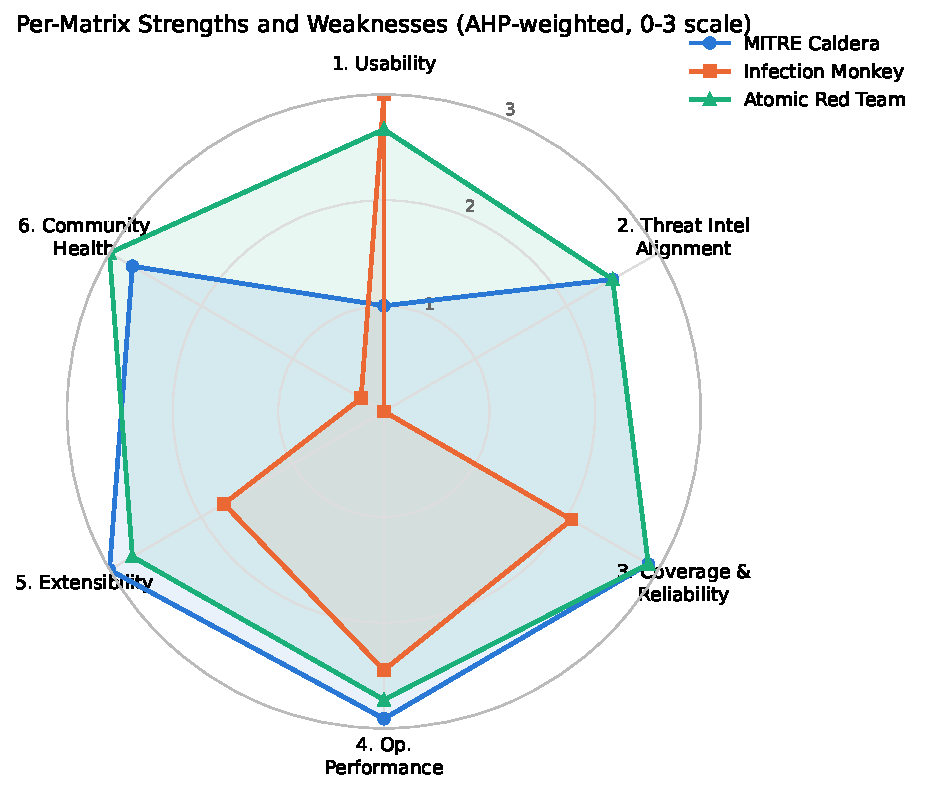
\includegraphics[width=0.75\textwidth]{figures/Figure_4_x_Spider_Chart.pdf}
\caption{Per-matrix strengths and weaknesses of the three BAS frameworks, using AHP-weighted within-matrix sub-criteria scores (0--3 scale). No single overall ranking is asserted: the chart is intended to show each tool's comparative strengths and weaknesses across the six evaluation dimensions rather than to declare one tool categorically ``best.''}
\label{fig:spider_chart}
\end{figure}




















